% Created by tikzDevice version 0.12.5 on 2024-01-20 15:03:01
% !TEX encoding = UTF-8 Unicode
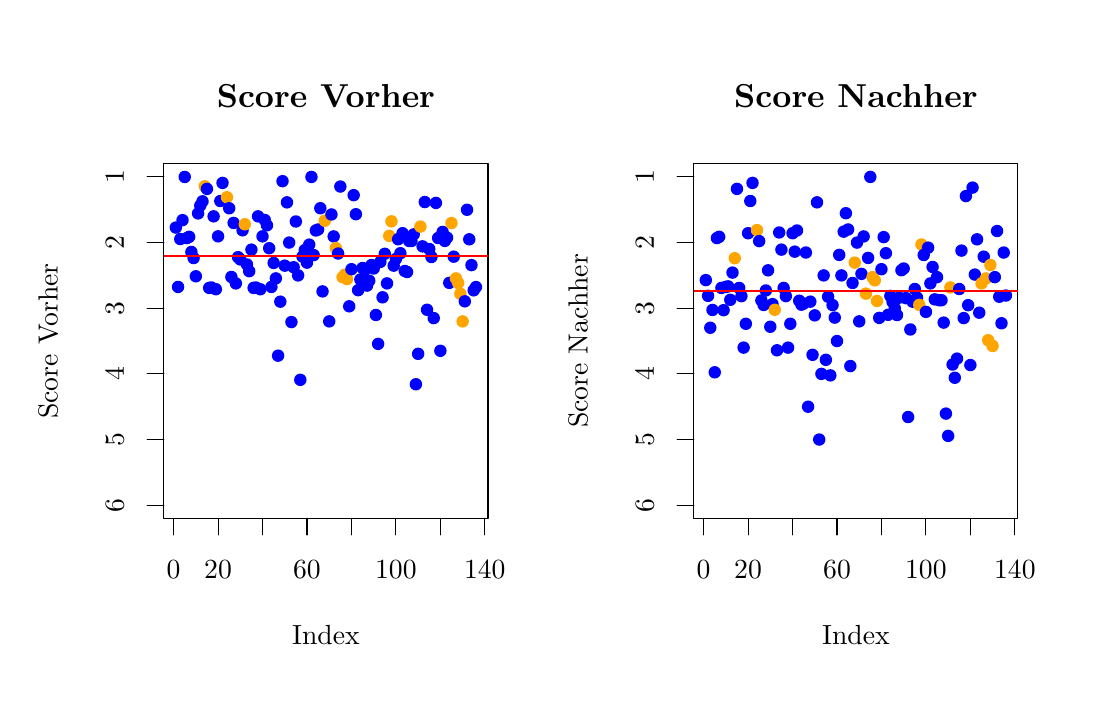
\begin{tikzpicture}[x=1pt,y=1pt]
\definecolor{fillColor}{RGB}{255,255,255}
\path[use as bounding box,fill=fillColor,fill opacity=0.00] (0,0) rectangle (383.03,238.49);
\begin{scope}
\path[clip] ( 49.20, 61.20) rectangle (166.32,189.29);
\definecolor{fillColor}{RGB}{0,0,255}

\path[fill=fillColor] ( 53.54,166.25) circle (  2.25);

\path[fill=fillColor] ( 54.34,144.80) circle (  2.25);

\path[fill=fillColor] ( 55.14,162.11) circle (  2.25);

\path[fill=fillColor] ( 55.95,168.94) circle (  2.25);

\path[fill=fillColor] ( 56.75,184.55) circle (  2.25);

\path[fill=fillColor] ( 57.55,162.46) circle (  2.25);

\path[fill=fillColor] ( 58.36,162.92) circle (  2.25);

\path[fill=fillColor] ( 59.16,157.44) circle (  2.25);

\path[fill=fillColor] ( 59.96,155.25) circle (  2.25);

\path[fill=fillColor] ( 60.77,148.65) circle (  2.25);

\path[fill=fillColor] ( 61.57,171.37) circle (  2.25);

\path[fill=fillColor] ( 62.37,174.21) circle (  2.25);

\path[fill=fillColor] ( 63.18,175.74) circle (  2.25);
\definecolor{fillColor}{RGB}{255,165,0}

\path[fill=fillColor] ( 63.98,181.16) circle (  2.25);
\definecolor{fillColor}{RGB}{0,0,255}

\path[fill=fillColor] ( 64.78,180.23) circle (  2.25);

\path[fill=fillColor] ( 65.59,144.45) circle (  2.25);

\path[fill=fillColor] ( 66.39,144.60) circle (  2.25);

\path[fill=fillColor] ( 67.19,170.31) circle (  2.25);

\path[fill=fillColor] ( 68.00,143.97) circle (  2.25);

\path[fill=fillColor] ( 68.80,163.09) circle (  2.25);

\path[fill=fillColor] ( 69.60,175.85) circle (  2.25);

\path[fill=fillColor] ( 70.41,182.39) circle (  2.25);
\definecolor{fillColor}{RGB}{255,165,0}

\path[fill=fillColor] ( 72.01,177.20) circle (  2.25);
\definecolor{fillColor}{RGB}{0,0,255}

\path[fill=fillColor] ( 72.82,173.23) circle (  2.25);

\path[fill=fillColor] ( 73.62,148.40) circle (  2.25);

\path[fill=fillColor] ( 74.42,167.94) circle (  2.25);

\path[fill=fillColor] ( 75.23,146.08) circle (  2.25);

\path[fill=fillColor] ( 76.03,155.56) circle (  2.25);

\path[fill=fillColor] ( 76.83,154.74) circle (  2.25);

\path[fill=fillColor] ( 77.64,165.27) circle (  2.25);
\definecolor{fillColor}{RGB}{255,165,0}

\path[fill=fillColor] ( 78.44,167.45) circle (  2.25);
\definecolor{fillColor}{RGB}{0,0,255}

\path[fill=fillColor] ( 79.24,152.92) circle (  2.25);

\path[fill=fillColor] ( 80.05,150.49) circle (  2.25);

\path[fill=fillColor] ( 80.85,158.28) circle (  2.25);

\path[fill=fillColor] ( 81.65,144.45) circle (  2.25);

\path[fill=fillColor] ( 82.46,144.60) circle (  2.25);

\path[fill=fillColor] ( 83.26,170.31) circle (  2.25);

\path[fill=fillColor] ( 84.06,143.97) circle (  2.25);

\path[fill=fillColor] ( 84.86,163.09) circle (  2.25);

\path[fill=fillColor] ( 85.67,169.01) circle (  2.25);

\path[fill=fillColor] ( 86.47,167.07) circle (  2.25);

\path[fill=fillColor] ( 87.27,158.79) circle (  2.25);

\path[fill=fillColor] ( 88.08,144.80) circle (  2.25);

\path[fill=fillColor] ( 88.88,153.48) circle (  2.25);

\path[fill=fillColor] ( 89.68,147.89) circle (  2.25);

\path[fill=fillColor] ( 90.49,119.97) circle (  2.25);

\path[fill=fillColor] ( 91.29,139.48) circle (  2.25);

\path[fill=fillColor] ( 92.09,183.02) circle (  2.25);

\path[fill=fillColor] ( 92.90,152.49) circle (  2.25);

\path[fill=fillColor] ( 93.70,175.36) circle (  2.25);

\path[fill=fillColor] ( 94.50,160.83) circle (  2.25);

\path[fill=fillColor] ( 95.31,132.11) circle (  2.25);

\path[fill=fillColor] ( 96.11,151.93) circle (  2.25);

\path[fill=fillColor] ( 96.91,168.45) circle (  2.25);

\path[fill=fillColor] ( 97.72,148.97) circle (  2.25);

\path[fill=fillColor] ( 98.52,111.23) circle (  2.25);

\path[fill=fillColor] ( 99.32,155.74) circle (  2.25);

\path[fill=fillColor] (100.13,158.12) circle (  2.25);

\path[fill=fillColor] (100.93,153.58) circle (  2.25);

\path[fill=fillColor] (101.73,160.09) circle (  2.25);

\path[fill=fillColor] (102.54,184.55) circle (  2.25);

\path[fill=fillColor] (103.34,156.31) circle (  2.25);

\path[fill=fillColor] (104.14,165.20) circle (  2.25);

\path[fill=fillColor] (104.95,165.57) circle (  2.25);

\path[fill=fillColor] (105.75,173.25) circle (  2.25);

\path[fill=fillColor] (106.55,143.19) circle (  2.25);
\definecolor{fillColor}{RGB}{255,165,0}

\path[fill=fillColor] (107.36,168.73) circle (  2.25);
\definecolor{fillColor}{RGB}{0,0,255}

\path[fill=fillColor] (108.96,132.36) circle (  2.25);

\path[fill=fillColor] (109.77,170.99) circle (  2.25);

\path[fill=fillColor] (110.57,163.05) circle (  2.25);
\definecolor{fillColor}{RGB}{255,165,0}

\path[fill=fillColor] (111.37,158.85) circle (  2.25);
\definecolor{fillColor}{RGB}{0,0,255}

\path[fill=fillColor] (112.18,156.87) circle (  2.25);

\path[fill=fillColor] (112.98,181.08) circle (  2.25);
\definecolor{fillColor}{RGB}{255,165,0}

\path[fill=fillColor] (113.78,148.34) circle (  2.25);

\path[fill=fillColor] (114.59,149.22) circle (  2.25);

\path[fill=fillColor] (115.39,147.65) circle (  2.25);
\definecolor{fillColor}{RGB}{0,0,255}

\path[fill=fillColor] (116.19,137.80) circle (  2.25);

\path[fill=fillColor] (117.00,151.21) circle (  2.25);

\path[fill=fillColor] (117.80,177.96) circle (  2.25);

\path[fill=fillColor] (118.60,171.08) circle (  2.25);

\path[fill=fillColor] (119.41,143.63) circle (  2.25);

\path[fill=fillColor] (120.21,147.48) circle (  2.25);

\path[fill=fillColor] (121.01,151.64) circle (  2.25);

\path[fill=fillColor] (121.81,150.94) circle (  2.25);

\path[fill=fillColor] (122.62,145.29) circle (  2.25);

\path[fill=fillColor] (123.42,147.05) circle (  2.25);

\path[fill=fillColor] (124.22,152.71) circle (  2.25);

\path[fill=fillColor] (125.03,151.46) circle (  2.25);

\path[fill=fillColor] (125.83,134.67) circle (  2.25);

\path[fill=fillColor] (126.63,124.23) circle (  2.25);

\path[fill=fillColor] (127.44,153.85) circle (  2.25);

\path[fill=fillColor] (128.24,141.06) circle (  2.25);

\path[fill=fillColor] (129.04,156.78) circle (  2.25);

\path[fill=fillColor] (129.85,146.08) circle (  2.25);
\definecolor{fillColor}{RGB}{255,165,0}

\path[fill=fillColor] (130.65,163.26) circle (  2.25);

\path[fill=fillColor] (131.45,168.50) circle (  2.25);
\definecolor{fillColor}{RGB}{0,0,255}

\path[fill=fillColor] (132.26,152.49) circle (  2.25);

\path[fill=fillColor] (133.06,154.90) circle (  2.25);

\path[fill=fillColor] (133.86,162.04) circle (  2.25);

\path[fill=fillColor] (134.67,156.98) circle (  2.25);

\path[fill=fillColor] (135.47,164.21) circle (  2.25);

\path[fill=fillColor] (136.27,150.57) circle (  2.25);

\path[fill=fillColor] (137.08,150.21) circle (  2.25);

\path[fill=fillColor] (137.88,161.40) circle (  2.25);

\path[fill=fillColor] (138.68,161.40) circle (  2.25);

\path[fill=fillColor] (139.49,163.79) circle (  2.25);

\path[fill=fillColor] (140.29,109.64) circle (  2.25);

\path[fill=fillColor] (141.09,120.63) circle (  2.25);
\definecolor{fillColor}{RGB}{255,165,0}

\path[fill=fillColor] (141.90,166.61) circle (  2.25);
\definecolor{fillColor}{RGB}{0,0,255}

\path[fill=fillColor] (142.70,159.47) circle (  2.25);

\path[fill=fillColor] (143.50,175.48) circle (  2.25);

\path[fill=fillColor] (144.31,136.55) circle (  2.25);

\path[fill=fillColor] (145.11,158.51) circle (  2.25);

\path[fill=fillColor] (145.91,155.62) circle (  2.25);

\path[fill=fillColor] (146.72,133.55) circle (  2.25);

\path[fill=fillColor] (147.52,175.16) circle (  2.25);

\path[fill=fillColor] (148.32,162.48) circle (  2.25);

\path[fill=fillColor] (149.13,121.72) circle (  2.25);

\path[fill=fillColor] (149.93,164.67) circle (  2.25);

\path[fill=fillColor] (150.73,161.43) circle (  2.25);

\path[fill=fillColor] (151.54,162.61) circle (  2.25);

\path[fill=fillColor] (152.34,146.27) circle (  2.25);
\definecolor{fillColor}{RGB}{255,165,0}

\path[fill=fillColor] (153.14,167.88) circle (  2.25);
\definecolor{fillColor}{RGB}{0,0,255}

\path[fill=fillColor] (153.95,155.74) circle (  2.25);
\definecolor{fillColor}{RGB}{255,165,0}

\path[fill=fillColor] (154.75,147.89) circle (  2.25);

\path[fill=fillColor] (155.55,146.23) circle (  2.25);

\path[fill=fillColor] (156.36,142.31) circle (  2.25);

\path[fill=fillColor] (157.16,132.36) circle (  2.25);
\definecolor{fillColor}{RGB}{0,0,255}

\path[fill=fillColor] (157.96,139.60) circle (  2.25);

\path[fill=fillColor] (158.76,172.69) circle (  2.25);

\path[fill=fillColor] (159.57,162.01) circle (  2.25);

\path[fill=fillColor] (160.37,152.69) circle (  2.25);

\path[fill=fillColor] (161.17,143.58) circle (  2.25);

\path[fill=fillColor] (161.98,144.76) circle (  2.25);
\end{scope}
\begin{scope}
\path[clip] (  0.00,  0.00) rectangle (383.03,238.49);
\definecolor{drawColor}{RGB}{0,0,0}

\path[draw=drawColor,line width= 0.4pt,line join=round,line cap=round] ( 52.73, 61.20) -- (165.19, 61.20);

\path[draw=drawColor,line width= 0.4pt,line join=round,line cap=round] ( 52.73, 61.20) -- ( 52.73, 55.20);

\path[draw=drawColor,line width= 0.4pt,line join=round,line cap=round] ( 68.80, 61.20) -- ( 68.80, 55.20);

\path[draw=drawColor,line width= 0.4pt,line join=round,line cap=round] ( 84.86, 61.20) -- ( 84.86, 55.20);

\path[draw=drawColor,line width= 0.4pt,line join=round,line cap=round] (100.93, 61.20) -- (100.93, 55.20);

\path[draw=drawColor,line width= 0.4pt,line join=round,line cap=round] (117.00, 61.20) -- (117.00, 55.20);

\path[draw=drawColor,line width= 0.4pt,line join=round,line cap=round] (133.06, 61.20) -- (133.06, 55.20);

\path[draw=drawColor,line width= 0.4pt,line join=round,line cap=round] (149.13, 61.20) -- (149.13, 55.20);

\path[draw=drawColor,line width= 0.4pt,line join=round,line cap=round] (165.19, 61.20) -- (165.19, 55.20);

\node[text=drawColor,anchor=base,inner sep=0pt, outer sep=0pt, scale=  1.00] at ( 52.73, 39.60) {0};

\node[text=drawColor,anchor=base,inner sep=0pt, outer sep=0pt, scale=  1.00] at ( 68.80, 39.60) {20};

\node[text=drawColor,anchor=base,inner sep=0pt, outer sep=0pt, scale=  1.00] at (100.93, 39.60) {60};

\node[text=drawColor,anchor=base,inner sep=0pt, outer sep=0pt, scale=  1.00] at (133.06, 39.60) {100};

\node[text=drawColor,anchor=base,inner sep=0pt, outer sep=0pt, scale=  1.00] at (165.19, 39.60) {140};

\path[draw=drawColor,line width= 0.4pt,line join=round,line cap=round] ( 49.20,184.55) -- ( 49.20, 65.94);

\path[draw=drawColor,line width= 0.4pt,line join=round,line cap=round] ( 49.20,184.55) -- ( 43.20,184.55);

\path[draw=drawColor,line width= 0.4pt,line join=round,line cap=round] ( 49.20,160.83) -- ( 43.20,160.83);

\path[draw=drawColor,line width= 0.4pt,line join=round,line cap=round] ( 49.20,137.11) -- ( 43.20,137.11);

\path[draw=drawColor,line width= 0.4pt,line join=round,line cap=round] ( 49.20,113.39) -- ( 43.20,113.39);

\path[draw=drawColor,line width= 0.4pt,line join=round,line cap=round] ( 49.20, 89.66) -- ( 43.20, 89.66);

\path[draw=drawColor,line width= 0.4pt,line join=round,line cap=round] ( 49.20, 65.94) -- ( 43.20, 65.94);

\node[text=drawColor,rotate= 90.00,anchor=base,inner sep=0pt, outer sep=0pt, scale=  1.00] at ( 34.80, 65.94) {6};

\node[text=drawColor,rotate= 90.00,anchor=base,inner sep=0pt, outer sep=0pt, scale=  1.00] at ( 34.80, 89.66) {5};

\node[text=drawColor,rotate= 90.00,anchor=base,inner sep=0pt, outer sep=0pt, scale=  1.00] at ( 34.80,113.39) {4};

\node[text=drawColor,rotate= 90.00,anchor=base,inner sep=0pt, outer sep=0pt, scale=  1.00] at ( 34.80,137.11) {3};

\node[text=drawColor,rotate= 90.00,anchor=base,inner sep=0pt, outer sep=0pt, scale=  1.00] at ( 34.80,160.83) {2};

\node[text=drawColor,rotate= 90.00,anchor=base,inner sep=0pt, outer sep=0pt, scale=  1.00] at ( 34.80,184.55) {1};

\path[draw=drawColor,line width= 0.4pt,line join=round,line cap=round] ( 49.20, 61.20) --
	(166.32, 61.20) --
	(166.32,189.29) --
	( 49.20,189.29) --
	cycle;
\end{scope}
\begin{scope}
\path[clip] (  0.00,  0.00) rectangle (191.52,238.49);
\definecolor{drawColor}{RGB}{0,0,0}

\node[text=drawColor,anchor=base,inner sep=0pt, outer sep=0pt, scale=  1.20] at (107.76,209.75) {\bfseries Score Vorher};

\node[text=drawColor,anchor=base,inner sep=0pt, outer sep=0pt, scale=  1.00] at (107.76, 15.60) {Index};

\node[text=drawColor,rotate= 90.00,anchor=base,inner sep=0pt, outer sep=0pt, scale=  1.00] at ( 10.80,125.25) {Score Vorher};
\end{scope}
\begin{scope}
\path[clip] ( 49.20, 61.20) rectangle (166.32,189.29);
\definecolor{drawColor}{RGB}{255,0,0}

\path[draw=drawColor,line width= 0.8pt,line join=round,line cap=round] ( 49.20,155.93) -- (166.32,155.93);
\end{scope}
\begin{scope}
\path[clip] (240.72, 61.20) rectangle (357.83,189.29);
\definecolor{fillColor}{RGB}{0,0,255}

\path[fill=fillColor] (245.05,147.27) circle (  2.25);

\path[fill=fillColor] (245.86,141.59) circle (  2.25);

\path[fill=fillColor] (246.66,130.05) circle (  2.25);

\path[fill=fillColor] (247.46,136.48) circle (  2.25);

\path[fill=fillColor] (248.27,113.95) circle (  2.25);

\path[fill=fillColor] (249.07,162.46) circle (  2.25);

\path[fill=fillColor] (249.87,162.92) circle (  2.25);

\path[fill=fillColor] (250.68,144.45) circle (  2.25);

\path[fill=fillColor] (251.48,136.41) circle (  2.25);

\path[fill=fillColor] (252.28,144.80) circle (  2.25);

\path[fill=fillColor] (253.09,145.01) circle (  2.25);

\path[fill=fillColor] (253.89,140.15) circle (  2.25);

\path[fill=fillColor] (254.69,149.98) circle (  2.25);
\definecolor{fillColor}{RGB}{255,165,0}

\path[fill=fillColor] (255.50,155.18) circle (  2.25);
\definecolor{fillColor}{RGB}{0,0,255}

\path[fill=fillColor] (256.30,180.23) circle (  2.25);

\path[fill=fillColor] (257.10,144.45) circle (  2.25);

\path[fill=fillColor] (257.91,141.48) circle (  2.25);

\path[fill=fillColor] (258.71,122.87) circle (  2.25);

\path[fill=fillColor] (259.51,131.49) circle (  2.25);

\path[fill=fillColor] (260.32,164.21) circle (  2.25);

\path[fill=fillColor] (261.12,175.85) circle (  2.25);

\path[fill=fillColor] (261.92,182.39) circle (  2.25);
\definecolor{fillColor}{RGB}{255,165,0}

\path[fill=fillColor] (263.53,165.34) circle (  2.25);
\definecolor{fillColor}{RGB}{0,0,255}

\path[fill=fillColor] (264.33,161.37) circle (  2.25);

\path[fill=fillColor] (265.13,139.93) circle (  2.25);

\path[fill=fillColor] (265.94,138.29) circle (  2.25);

\path[fill=fillColor] (266.74,143.52) circle (  2.25);

\path[fill=fillColor] (267.54,150.81) circle (  2.25);

\path[fill=fillColor] (268.35,130.42) circle (  2.25);

\path[fill=fillColor] (269.15,138.59) circle (  2.25);
\definecolor{fillColor}{RGB}{255,165,0}

\path[fill=fillColor] (269.95,136.55) circle (  2.25);
\definecolor{fillColor}{RGB}{0,0,255}

\path[fill=fillColor] (270.76,121.90) circle (  2.25);

\path[fill=fillColor] (271.56,164.48) circle (  2.25);

\path[fill=fillColor] (272.36,158.28) circle (  2.25);

\path[fill=fillColor] (273.17,144.45) circle (  2.25);

\path[fill=fillColor] (273.97,141.48) circle (  2.25);

\path[fill=fillColor] (274.77,122.87) circle (  2.25);

\path[fill=fillColor] (275.58,131.49) circle (  2.25);

\path[fill=fillColor] (276.38,164.21) circle (  2.25);

\path[fill=fillColor] (277.18,157.55) circle (  2.25);

\path[fill=fillColor] (277.99,165.20) circle (  2.25);

\path[fill=fillColor] (278.79,139.82) circle (  2.25);

\path[fill=fillColor] (279.59,138.39) circle (  2.25);

\path[fill=fillColor] (280.40,138.80) circle (  2.25);

\path[fill=fillColor] (281.20,157.23) circle (  2.25);

\path[fill=fillColor] (282.00,101.52) circle (  2.25);

\path[fill=fillColor] (282.81,139.48) circle (  2.25);

\path[fill=fillColor] (283.61,120.27) circle (  2.25);

\path[fill=fillColor] (284.41,134.54) circle (  2.25);

\path[fill=fillColor] (285.22,175.36) circle (  2.25);

\path[fill=fillColor] (286.02, 89.66) circle (  2.25);

\path[fill=fillColor] (286.82,113.39) circle (  2.25);

\path[fill=fillColor] (287.63,148.97) circle (  2.25);

\path[fill=fillColor] (288.43,118.47) circle (  2.25);

\path[fill=fillColor] (289.23,141.26) circle (  2.25);

\path[fill=fillColor] (290.04,112.85) circle (  2.25);

\path[fill=fillColor] (290.84,138.24) circle (  2.25);

\path[fill=fillColor] (291.64,133.72) circle (  2.25);

\path[fill=fillColor] (292.45,125.25) circle (  2.25);

\path[fill=fillColor] (293.25,156.38) circle (  2.25);

\path[fill=fillColor] (294.05,148.97) circle (  2.25);

\path[fill=fillColor] (294.86,164.78) circle (  2.25);

\path[fill=fillColor] (295.66,171.44) circle (  2.25);

\path[fill=fillColor] (296.46,165.57) circle (  2.25);

\path[fill=fillColor] (297.27,116.21) circle (  2.25);

\path[fill=fillColor] (298.07,146.23) circle (  2.25);
\definecolor{fillColor}{RGB}{255,165,0}

\path[fill=fillColor] (298.87,153.58) circle (  2.25);
\definecolor{fillColor}{RGB}{0,0,255}

\path[fill=fillColor] (299.67,160.83) circle (  2.25);

\path[fill=fillColor] (300.48,132.36) circle (  2.25);

\path[fill=fillColor] (301.28,149.53) circle (  2.25);

\path[fill=fillColor] (302.08,163.05) circle (  2.25);
\definecolor{fillColor}{RGB}{255,165,0}

\path[fill=fillColor] (302.89,142.38) circle (  2.25);
\definecolor{fillColor}{RGB}{0,0,255}

\path[fill=fillColor] (303.69,155.29) circle (  2.25);

\path[fill=fillColor] (304.49,184.55) circle (  2.25);
\definecolor{fillColor}{RGB}{255,165,0}

\path[fill=fillColor] (305.30,148.34) circle (  2.25);

\path[fill=fillColor] (306.10,147.20) circle (  2.25);

\path[fill=fillColor] (306.90,139.74) circle (  2.25);
\definecolor{fillColor}{RGB}{0,0,255}

\path[fill=fillColor] (307.71,133.62) circle (  2.25);

\path[fill=fillColor] (308.51,151.21) circle (  2.25);

\path[fill=fillColor] (309.31,162.80) circle (  2.25);

\path[fill=fillColor] (310.12,156.98) circle (  2.25);

\path[fill=fillColor] (310.92,134.73) circle (  2.25);

\path[fill=fillColor] (311.72,141.55) circle (  2.25);

\path[fill=fillColor] (312.53,139.40) circle (  2.25);

\path[fill=fillColor] (313.33,137.11) circle (  2.25);

\path[fill=fillColor] (314.13,134.65) circle (  2.25);

\path[fill=fillColor] (314.94,140.93) circle (  2.25);

\path[fill=fillColor] (315.74,150.84) circle (  2.25);

\path[fill=fillColor] (316.54,151.46) circle (  2.25);

\path[fill=fillColor] (317.35,140.76) circle (  2.25);

\path[fill=fillColor] (318.15, 97.80) circle (  2.25);

\path[fill=fillColor] (318.95,129.43) circle (  2.25);

\path[fill=fillColor] (319.76,139.48) circle (  2.25);

\path[fill=fillColor] (320.56,144.05) circle (  2.25);

\path[fill=fillColor] (321.36,140.95) circle (  2.25);
\definecolor{fillColor}{RGB}{255,165,0}

\path[fill=fillColor] (322.17,138.32) circle (  2.25);

\path[fill=fillColor] (322.97,160.13) circle (  2.25);
\definecolor{fillColor}{RGB}{0,0,255}

\path[fill=fillColor] (323.77,156.34) circle (  2.25);

\path[fill=fillColor] (324.58,135.79) circle (  2.25);

\path[fill=fillColor] (325.38,159.00) circle (  2.25);

\path[fill=fillColor] (326.18,146.08) circle (  2.25);

\path[fill=fillColor] (326.99,152.02) circle (  2.25);

\path[fill=fillColor] (327.79,140.31) circle (  2.25);

\path[fill=fillColor] (328.59,148.34) circle (  2.25);

\path[fill=fillColor] (329.40,140.00) circle (  2.25);

\path[fill=fillColor] (330.20,140.00) circle (  2.25);

\path[fill=fillColor] (331.00,131.92) circle (  2.25);

\path[fill=fillColor] (331.81, 99.03) circle (  2.25);

\path[fill=fillColor] (332.61, 90.98) circle (  2.25);
\definecolor{fillColor}{RGB}{255,165,0}

\path[fill=fillColor] (333.41,144.63) circle (  2.25);
\definecolor{fillColor}{RGB}{0,0,255}

\path[fill=fillColor] (334.22,116.77) circle (  2.25);

\path[fill=fillColor] (335.02,111.99) circle (  2.25);

\path[fill=fillColor] (335.82,118.90) circle (  2.25);

\path[fill=fillColor] (336.62,144.05) circle (  2.25);

\path[fill=fillColor] (337.43,157.93) circle (  2.25);

\path[fill=fillColor] (338.23,133.55) circle (  2.25);

\path[fill=fillColor] (339.03,177.63) circle (  2.25);

\path[fill=fillColor] (339.84,138.21) circle (  2.25);

\path[fill=fillColor] (340.64,116.59) circle (  2.25);

\path[fill=fillColor] (341.44,180.70) circle (  2.25);

\path[fill=fillColor] (342.25,149.27) circle (  2.25);

\path[fill=fillColor] (343.05,162.01) circle (  2.25);

\path[fill=fillColor] (343.85,135.49) circle (  2.25);
\definecolor{fillColor}{RGB}{255,165,0}

\path[fill=fillColor] (344.66,146.08) circle (  2.25);
\definecolor{fillColor}{RGB}{0,0,255}

\path[fill=fillColor] (345.46,155.74) circle (  2.25);
\definecolor{fillColor}{RGB}{255,165,0}

\path[fill=fillColor] (346.26,147.89) circle (  2.25);

\path[fill=fillColor] (347.07,125.55) circle (  2.25);

\path[fill=fillColor] (347.87,152.73) circle (  2.25);

\path[fill=fillColor] (348.67,123.47) circle (  2.25);
\definecolor{fillColor}{RGB}{0,0,255}

\path[fill=fillColor] (349.48,148.34) circle (  2.25);

\path[fill=fillColor] (350.28,165.01) circle (  2.25);

\path[fill=fillColor] (351.08,141.26) circle (  2.25);

\path[fill=fillColor] (351.89,131.68) circle (  2.25);

\path[fill=fillColor] (352.69,157.23) circle (  2.25);

\path[fill=fillColor] (353.49,141.70) circle (  2.25);
\end{scope}
\begin{scope}
\path[clip] (  0.00,  0.00) rectangle (383.03,238.49);
\definecolor{drawColor}{RGB}{0,0,0}

\path[draw=drawColor,line width= 0.4pt,line join=round,line cap=round] (244.25, 61.20) -- (356.71, 61.20);

\path[draw=drawColor,line width= 0.4pt,line join=round,line cap=round] (244.25, 61.20) -- (244.25, 55.20);

\path[draw=drawColor,line width= 0.4pt,line join=round,line cap=round] (260.32, 61.20) -- (260.32, 55.20);

\path[draw=drawColor,line width= 0.4pt,line join=round,line cap=round] (276.38, 61.20) -- (276.38, 55.20);

\path[draw=drawColor,line width= 0.4pt,line join=round,line cap=round] (292.45, 61.20) -- (292.45, 55.20);

\path[draw=drawColor,line width= 0.4pt,line join=round,line cap=round] (308.51, 61.20) -- (308.51, 55.20);

\path[draw=drawColor,line width= 0.4pt,line join=round,line cap=round] (324.58, 61.20) -- (324.58, 55.20);

\path[draw=drawColor,line width= 0.4pt,line join=round,line cap=round] (340.64, 61.20) -- (340.64, 55.20);

\path[draw=drawColor,line width= 0.4pt,line join=round,line cap=round] (356.71, 61.20) -- (356.71, 55.20);

\node[text=drawColor,anchor=base,inner sep=0pt, outer sep=0pt, scale=  1.00] at (244.25, 39.60) {0};

\node[text=drawColor,anchor=base,inner sep=0pt, outer sep=0pt, scale=  1.00] at (260.32, 39.60) {20};

\node[text=drawColor,anchor=base,inner sep=0pt, outer sep=0pt, scale=  1.00] at (292.45, 39.60) {60};

\node[text=drawColor,anchor=base,inner sep=0pt, outer sep=0pt, scale=  1.00] at (324.58, 39.60) {100};

\node[text=drawColor,anchor=base,inner sep=0pt, outer sep=0pt, scale=  1.00] at (356.71, 39.60) {140};

\path[draw=drawColor,line width= 0.4pt,line join=round,line cap=round] (240.72,184.55) -- (240.72, 65.94);

\path[draw=drawColor,line width= 0.4pt,line join=round,line cap=round] (240.72,184.55) -- (234.72,184.55);

\path[draw=drawColor,line width= 0.4pt,line join=round,line cap=round] (240.72,160.83) -- (234.72,160.83);

\path[draw=drawColor,line width= 0.4pt,line join=round,line cap=round] (240.72,137.11) -- (234.72,137.11);

\path[draw=drawColor,line width= 0.4pt,line join=round,line cap=round] (240.72,113.39) -- (234.72,113.39);

\path[draw=drawColor,line width= 0.4pt,line join=round,line cap=round] (240.72, 89.66) -- (234.72, 89.66);

\path[draw=drawColor,line width= 0.4pt,line join=round,line cap=round] (240.72, 65.94) -- (234.72, 65.94);

\node[text=drawColor,rotate= 90.00,anchor=base,inner sep=0pt, outer sep=0pt, scale=  1.00] at (226.32, 65.94) {6};

\node[text=drawColor,rotate= 90.00,anchor=base,inner sep=0pt, outer sep=0pt, scale=  1.00] at (226.32, 89.66) {5};

\node[text=drawColor,rotate= 90.00,anchor=base,inner sep=0pt, outer sep=0pt, scale=  1.00] at (226.32,113.39) {4};

\node[text=drawColor,rotate= 90.00,anchor=base,inner sep=0pt, outer sep=0pt, scale=  1.00] at (226.32,137.11) {3};

\node[text=drawColor,rotate= 90.00,anchor=base,inner sep=0pt, outer sep=0pt, scale=  1.00] at (226.32,160.83) {2};

\node[text=drawColor,rotate= 90.00,anchor=base,inner sep=0pt, outer sep=0pt, scale=  1.00] at (226.32,184.55) {1};

\path[draw=drawColor,line width= 0.4pt,line join=round,line cap=round] (240.72, 61.20) --
	(357.83, 61.20) --
	(357.83,189.29) --
	(240.72,189.29) --
	cycle;
\end{scope}
\begin{scope}
\path[clip] (191.52,  0.00) rectangle (383.03,238.49);
\definecolor{drawColor}{RGB}{0,0,0}

\node[text=drawColor,anchor=base,inner sep=0pt, outer sep=0pt, scale=  1.20] at (299.27,209.75) {\bfseries Score Nachher};

\node[text=drawColor,anchor=base,inner sep=0pt, outer sep=0pt, scale=  1.00] at (299.27, 15.60) {Index};

\node[text=drawColor,rotate= 90.00,anchor=base,inner sep=0pt, outer sep=0pt, scale=  1.00] at (202.32,125.25) {Score Nachher};
\end{scope}
\begin{scope}
\path[clip] (240.72, 61.20) rectangle (357.83,189.29);
\definecolor{drawColor}{RGB}{255,0,0}

\path[draw=drawColor,line width= 0.8pt,line join=round,line cap=round] (240.72,143.22) -- (357.83,143.22);
\end{scope}
\end{tikzpicture}
